% ------------------------------------------------------------------------------
% TYPO3 CMS 8.4 - What's New - Chapter "Deprecated Functions" (Serbian Version)
%
% @author	Michael Schams <schams.net>
% @license	Creative Commons BY-NC-SA 3.0
% @link		http://typo3.org/download/release-notes/whats-new/
% @language	English
% ------------------------------------------------------------------------------
% LTXE-CHAPTER-UID:		3f842373-9262b8d3-f9c8de76-cf29ce17
% LTXE-CHAPTER-NAME:	Deprecated Functions
% ------------------------------------------------------------------------------

\section{Deprecated/Removed Functions}
\begin{frame}[fragile]
	\frametitle{Deprecated/Removed Functions}

	\begin{center}\huge{Chapter 5:}\end{center}
	\begin{center}\huge{\color{typo3darkgrey}\textbf{Deprecated/Removed Functions}}\end{center}

\end{frame}

% ------------------------------------------------------------------------------
% LTXE-SLIDE-START
% LTXE-SLIDE-UID:		4ed6248a-b0ac19cf-2527d8e7-3da3b7b2
% LTXE-SLIDE-ORIGIN:	cf7400eb-0f683329-f6c51cbf-dfd192d9 English
% LTXE-SLIDE-TITLE:		#77630: Remove wizard icons
% ------------------------------------------------------------------------------
\begin{frame}[fragile]
	\frametitle{Deprecated/Removed Functions}
	\framesubtitle{Wizard Icons Removed}

	\begin{itemize}

		\item The following icons have been removed from the FormFieldWizard:

			\begin{itemize}
				\item \texttt{wizard\_add.gif}
				\item \texttt{wizard\_edit.gif}
				\item \texttt{wizard\_link.gif}
				\item \texttt{wizard\_list.gif}
				\item \texttt{wizard\_rte.gif}
				\item \texttt{wizard\_table.gif}
			\end{itemize}

	\end{itemize}

	\begin{figure}
		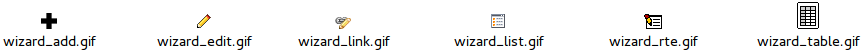
\includegraphics[width=0.95\linewidth]{DeprecatedRemovedFunctions/77630.png}
	\end{figure}

\end{frame}

% ------------------------------------------------------------------------------
% LTXE-SLIDE-START
% LTXE-SLIDE-UID:		7d2e2328-26bae9cf-faf733db-99a96c76
% LTXE-SLIDE-ORIGIN:	d5ced5e7-04dffe16-b8ec9f2c-712020cd English
% LTXE-SLIDE-TITLE:		#77693: Remove/Move Icons from EXT:t3skin
% ------------------------------------------------------------------------------

\begin{frame}[fragile]
	\frametitle{Deprecated/Removed Functions}
	\framesubtitle{Icons from \texttt{EXT:t3skin}}

	\begin{itemize}

		\item Icons from \texttt{EXT:t3skin} have been removed or moved
		\item \textbf{Removed:}

			\begin{itemize}
				\item \smaller\texttt{typo3/sysext/t3skin/icons/gfx/error.png}
				\item \texttt{typo3/sysext/t3skin/icons/gfx/i/\_icon\_ftp.gif}
				\item \texttt{typo3/sysext/t3skin/icons/gfx/information.png}
				\item \texttt{typo3/sysext/t3skin/icons/gfx/notice.png}
				\item \texttt{typo3/sysext/t3skin/icons/gfx/warning.png}
			\end{itemize}

		\item \textbf{Moved:}

			\begin{itemize}
				\item \smaller\texttt{typo3/sysext/t3skin/icons/gfx/icon\_fatalerror.gif}
				\item \texttt{typo3/sysext/t3skin/images/icons/status/status-edit-read-only.png}
				\item \texttt{typo3/sysext/t3skin/images/icons/status/warning-in-use.png}
				\item \texttt{typo3/sysext/t3skin/images/icons/status/warning-lock.png}
				\item \texttt{typo3/sysext/t3skin/images/icons/status/status-reference-hard.png}
				\item \texttt{typo3/sysext/t3skin/images/icons/status/status-reference-soft.png}
			\end{itemize}

	\end{itemize}

\end{frame}

% ------------------------------------------------------------------------------
% LTXE-SLIDE-START
% LTXE-SLIDE-UID:		3b8540af-34d0ec9f-bd921763-45aba814
% LTXE-SLIDE-ORIGIN:	7848f0b0-d687b337-f7638646-680dc819 English
% LTXE-SLIDE-TITLE:		Obsolete page tree and click menu settings removed
% ------------------------------------------------------------------------------

\begin{frame}[fragile]
	\frametitle{Deprecated/Removed Functions}
	\framesubtitle{Page tree and click menu settings}

	\begin{itemize}

		\item Obsolete page tree and click menu settings have been removed
		\item \textbf{Properties}:

		\begin{itemize}
			\item \texttt{FileSystemNavigationFrameController->doHighlight}
			\item \texttt{ClickMenu->leftIcons}
		\end{itemize}

		\item \textbf{TypoScript settings}:

		\begin{itemize}
			\item \texttt{options.pageTree.disableTitleHighlight}
			\item \texttt{options.contextMenu.options.leftIcons}
		\end{itemize}

	\end{itemize}

\end{frame}

% ------------------------------------------------------------------------------
% LTXE-SLIDE-START
% LTXE-SLIDE-UID:		3eba9879-6622372a-85258838-97adf207
% LTXE-SLIDE-ORIGIN:	aad23a73-7b046eaf-fb4bb862-2f88ef71 English
% LTXE-SLIDE-TITLE:		ExtensionManagementUtility::extRelPath()
% LTXE-SLIDE-REFERENCE:	#78193: ExtensionManagementUtility::extRelPath() deprecated
% ------------------------------------------------------------------------------

\begin{frame}[fragile]
	\frametitle{Deprecated/Removed Functions}
	\framesubtitle{ExtensionManagementUtility::extRelPath()}

	\begin{itemize}

		\item Method \texttt{ExtensionManagementUtility::extRelPath()} has been marked as deprecated
		\item This method was used to resolve paths relative to the current script
		\item Alternatives methods are available:

			\begin{itemize}
				\item \texttt{ExtensionManagementUtility::extPath()}\newline
					(to resolve the full path of an extension)
				\item \texttt{ExtensionManagementUtility::siteRelPath()}\newline
					(to resolve the location of an extension relative to \texttt{PATH\_site}
				\item \texttt{GeneralUtility::getFileAbsFileName()}\newline
					(to resolve a file/path prefixed with EXT:myextension
				\item \texttt{PathUtility::getAbsoluteWebPath()}\newline
					(to output a file location that is absolutely prefixed for the web folder)
			\end{itemize}

	\end{itemize}

\end{frame}

% ------------------------------------------------------------------------------
% LTXE-SLIDE-START
% LTXE-SLIDE-UID:		dd170cff-80c526bb-cfbc0939-faf00207
% LTXE-SLIDE-ORIGIN:	43a5eaf5-8945a8d5-ac27d4ea-24ffc8e3 English
% LTXE-SLIDE-TITLE:		Miscellaneous (1) (#75363)
% LTXE-SLIDE-REFERENCE:	#75363: Deprecate FormResultCompiler->JStop()
% LTXE-SLIDE-REFERENCE:	#75637: Deprecate optional parameters of RecyclerUtility::getRecordPath()
% ------------------------------------------------------------------------------

\begin{frame}[fragile]
	\frametitle{Deprecated/Removed Functions}
	\framesubtitle{Miscellaneous (1)}

	\begin{itemize}
		\item Method \texttt{FormResultCompiler->JStop()} has been renamed to \texttt{addCssFiles()}.
			The old method name is still present as a deprecated alias, which will be removed in TYPO3 v9.

		\item Method \texttt{ClickMenu::DB\_editPageProperties()} has been marked as deprecated

		\item The following arguments of method \texttt{RecyclerUtility::getRecordPath()} have been marked as deprecated:

			\begin{itemize}
				\item \texttt{\$clause}
				\item \texttt{\$titleLimit}
				\item \texttt{\$fullTitleLimit}
			\end{itemize}

	\end{itemize}

\end{frame}

% ------------------------------------------------------------------------------
% LTXE-SLIDE-START
% LTXE-SLIDE-UID:		603c2aed-94a86eec-c8041ffc-0b00a426
% LTXE-SLIDE-ORIGIN:	0745e3f3-83db03d7-ac24e92a-300391ba English
% LTXE-SLIDE-TITLE:		Miscellaneous (2) (#77783 and #77826)
% LTXE-SLIDE-REFERENCE:	#77783: Unused ExtJS JavaScript libraries removed
% LTXE-SLIDE-REFERENCE:	#77826: RTEHtmlArea Spellchecker eID removed
% ------------------------------------------------------------------------------

\begin{frame}[fragile]
	\frametitle{Deprecated/Removed Functions}
	\framesubtitle{Miscellaneous (2)}

	\begin{itemize}

		\item The following unused ExtJS JavaScript libraries have been removed:

			\begin{itemize}
				\item \texttt{app.SearchField}
				\item \texttt{grid.RowExpander}
				\item \texttt{ux.FitToParent}
			\end{itemize}

		\item RTEHtmlArea eID (\texttt{rtehtmlarea\_spellchecker}) for using
			dynamic spellchecking has been removed and entry point for HTTP Requests
			\texttt{SpellCheckingController->main} marked as deprecated

		\item Format \texttt{DateTime::ISO8601} is incompatible with ISO-8601,
			but is left for backward compatibility reasons.
			The constant \texttt{DateTime::ATOM} or \texttt{DATE\_ATOM} is used instead.

	\end{itemize}

\end{frame}

% ------------------------------------------------------------------------------
% LTXE-SLIDE-START
% LTXE-SLIDE-UID:		32891060-db852164-df344dcc-fdf72ea0
% LTXE-SLIDE-ORIGIN:	0745e3f3-83db03d7-ac24e92a-300391ba English
% LTXE-SLIDE-TITLE:		Miscellaneous (3) (#77839, #78096 and #78222)
% LTXE-SLIDE-REFERENCE:	#77839: TYPO3/CMS/Core/QueryGenerator
% LTXE-SLIDE-REFERENCE:	#78096: Deprecate PageLayoutView::getResult with mysqli_result objects
% LTXE-SLIDE-REFERENCE:	#78222: Late generation of autoload information is deprecated
% ------------------------------------------------------------------------------

\begin{frame}[fragile]
	\frametitle{Deprecated/Removed Functions}
	\framesubtitle{Miscellaneous (3)}

	\begin{itemize}

		\item AMD module \texttt{TYPO3/CMS/Core/QueryGenerator} has been moved to EXT:lowlevel\newline
			\small
				(and renamed to \texttt{TYPO3/CMS/Lowlevel/QueryGenerator})
			\normalsize

		\item Method \texttt{PageLayoutView::getResult()} has been marked as deprecated with
			the usage of \texttt{mysqli\_result} objects as first parameter

		\item If TYPO3 is in non-composer mode, it used to automatically dump extension class
			loading information late during the bootstrap. This behavior is deprecated now.
	\end{itemize}

\end{frame}

% ------------------------------------------------------------------------------
